\begin{figure}[H]
\centering
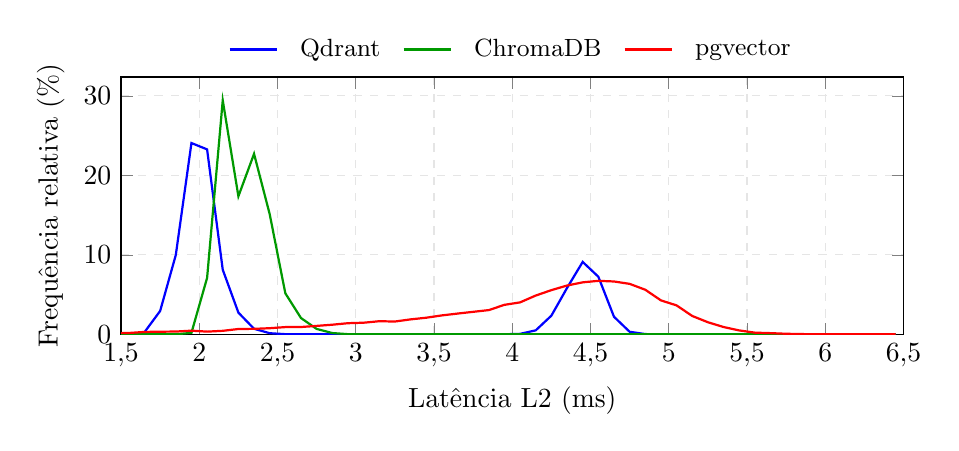
\begin{tikzpicture}
\begin{axis}[
    width=0.95\textwidth, height=0.40\textwidth,
    xlabel={Latência L2 (ms)}, ylabel={Frequência relativa (\%)},
    xmin=1.5, xmax=6.5, ymin=0,
    grid=major, grid style={dashed, gray!20},
    /pgf/number format/use comma,
    legend columns=3,
    legend style={at={(0.5,1.02)}, anchor=south, font=\small, draw=none, /tikz/column sep=6pt}
]
\addplot[color=blue, thick, mark=none] coordinates {
    (1.45, 0.00) (1.55, 0.00) (1.65, 0.27) (1.75, 2.94) (1.85, 9.98) (1.95, 24.07) (2.05, 23.27) (2.15, 8.13) (2.25, 2.73) (2.35, 0.70) (2.45, 0.14) (2.55, 0.02) (2.65, 0.01) (2.75, 0.01) (2.85, 0.01) (2.95, 0.01) (3.05, 0.01) (3.15, 0.00) (3.25, 0.01) (3.35, 0.01) (3.45, 0.01) (3.55, 0.00) (3.65, 0.00) (3.75, 0.00) (3.85, 0.00) (3.95, 0.01) (4.05, 0.06) (4.15, 0.50) (4.25, 2.35) (4.35, 5.83) (4.45, 9.11) (4.55, 7.25) (4.65, 2.21) (4.75, 0.32) (4.85, 0.03) (4.95, 0.00) (5.05, 0.00) (5.15, 0.00) (5.25, 0.00) (5.35, 0.00) (5.45, 0.00) (5.55, 0.00) (5.65, 0.00) (5.75, 0.00) (5.85, 0.00) (5.95, 0.00) (6.05, 0.00) (6.15, 0.00) (6.25, 0.00) (6.35, 0.00) (6.45, 0.00)
};
\addlegendentry{Qdrant}
\addplot[color=green!60!black, thick, mark=none] coordinates {
    (1.45, 0.00) (1.55, 0.00) (1.65, 0.00) (1.75, 0.00) (1.85, 0.00) (1.95, 0.19) (2.05, 7.10) (2.15, 29.44) (2.25, 17.37) (2.35, 22.71) (2.45, 15.12) (2.55, 5.16) (2.65, 2.05) (2.75, 0.68) (2.85, 0.16) (2.95, 0.02) (3.05, 0.01) (3.15, 0.00) (3.25, 0.00) (3.35, 0.00) (3.45, 0.00) (3.55, 0.00) (3.65, 0.00) (3.75, 0.00) (3.85, 0.00) (3.95, 0.00) (4.05, 0.00) (4.15, 0.00) (4.25, 0.00) (4.35, 0.00) (4.45, 0.00) (4.55, 0.00) (4.65, 0.00) (4.75, 0.00) (4.85, 0.00) (4.95, 0.00) (5.05, 0.00) (5.15, 0.00) (5.25, 0.00) (5.35, 0.00) (5.45, 0.00) (5.55, 0.00) (5.65, 0.00) (5.75, 0.00) (5.85, 0.00) (5.95, 0.00) (6.05, 0.00) (6.15, 0.00) (6.25, 0.00) (6.35, 0.00) (6.45, 0.00)
};
\addlegendentry{ChromaDB}
\addplot[color=red, thick, mark=none] coordinates {
    (1.45, 0.13) (1.55, 0.17) (1.65, 0.30) (1.75, 0.33) (1.85, 0.35) (1.95, 0.46) (2.05, 0.34) (2.15, 0.44) (2.25, 0.67) (2.35, 0.69) (2.45, 0.77) (2.55, 0.91) (2.65, 0.92) (2.75, 1.06) (2.85, 1.21) (2.95, 1.40) (3.05, 1.46) (3.15, 1.65) (3.25, 1.61) (3.35, 1.88) (3.45, 2.09) (3.55, 2.38) (3.65, 2.61) (3.75, 2.83) (3.85, 3.05) (3.95, 3.71) (4.05, 4.02) (4.15, 4.88) (4.25, 5.56) (4.35, 6.14) (4.45, 6.54) (4.55, 6.73) (4.65, 6.65) (4.75, 6.35) (4.85, 5.61) (4.95, 4.27) (5.05, 3.64) (5.15, 2.31) (5.25, 1.52) (5.35, 0.92) (5.45, 0.49) (5.55, 0.21) (5.65, 0.15) (5.75, 0.07) (5.85, 0.03) (5.95, 0.01) (6.05, 0.01) (6.15, 0.02) (6.25, 0.01) (6.35, 0.00) (6.45, 0.00)
};
\addlegendentry{pgvector}
\end{axis}
\end{tikzpicture}
\caption{Distribuição da latência para as consultas sequenciais sob a \textbf{Métrica L2}, agregando as \num{50000} consultas das 5 réplicas de cada motor (classes de 0,1~ms). Menos de 0,6\% das consultas, todas do pgvector e abaixo de 1,5~ms, ficam fora da janela representada.}
\label{fig:latencia_distribuicao_l2}
\end{figure}
